\documentclass[report.tex]{subfiles}

\begin{document}

\chapter{Literature Review and Research Proposal}

\section{Wearable and low-power application's constraints considerations}

\subsection{Constraints and challenges of low-power electronics}
Small embedded and wearable electronic systems had to overcome several constraints and challenges to become so popular and to take such a prominent place in everyone's daily life.\\

Challenges and constraints as follows:
\begin{itemize}
\item \textbf{Mechanical:}
\begin{itemize}
\item Increase portability by reducing internal electronic clutter and optimizing circuit complexity in order to increase component density and reduce weight as much as possible.
\item Improve ergonomics and design by increasing size and accessibility of user interface components like display, touch-screen or buttons.
\end{itemize}
\item \textbf{Performance:}
\begin{itemize}
\item Increase systems battery life as much as possible by reducing wasted power such as \textit{quiescent current} ($I_q$) and component efficiency, also in terms of heat dissipation which must be kept as low as possible in order to maintain a reasonable system temperature with a passive cooling design and does not reduce system performance by thermally throttling ICs or reducing battery cell capacity and efficiency. Each \si{\mu\ampere} should be dedicated to the system performance.
\item Reduce charging time as low as possible by increasing charging current as much as possible and choosing new technologies; such as \textit{USB-C PD}.
\end{itemize}
\item \textbf{Price and availability:}
\begin{itemize}
\item Reduce price of the system and increase the ease of production by reducing the number of components and optimizing the system complexity.\\
\end{itemize}
\end{itemize}

Designing ultra-low-power electronics is a constant trade-off between performance and battery autonomy.
A good approach consist in reducing as much as possible all sources of wasted currents and more precisely quiescent current.

\pagebreak

\subsubsection{Quiescent current ($I_Q$)}

The following description is based on the paper \textit{"Overcoming Low-IQ Challenges in
Low-Power Applications"}\cite{lowIqApp} by \textbf{Keith Kunz} and \textbf{Stefan Reithmaier} from \textsc{Texas Instrument Incorporated} and \textit{IQ: What it is, what it isn’t, and how to use it}\cite{IqIntro} by \textbf{Chris Glaser} from \textsc{Texas Instrument Incorporated}.\\

The \textit{quiescent current} ($I_Q$) is the current drown by an \textbf{active} IC when \textbf{non-switching} and a \textbf{no-load} configuration. 
\begin{itemize}
\item \textbf{Active} means that the IC is enabled and is neither in lockout nor shut-down condition. 
\item \textbf{No-load} means that not any current is drawn by the outputs of the IC. $I_Q$ is therefore all currents travelling inside the IC to the ground. 
\item \textbf{Non-switching} means that the IC is in a \textit{high-impedance} state, with its power stage disconnected from any output.
\end{itemize}

\section{System MCU - \textit{nRF9160 SiP}\cite{nrf9160brief} (\textsc{Nordi Semiconductor})}

\subsection{Overview}

The \textit{nRF9160 SiP} product bief: "\textit{nRF9160 cellular IoT System-in-Package}"\cite{nrf9160brief} describe the SiP as follows:
\begin{enumerate}
\item Accessible \textit{LTE} lates technology
\item Fully integrated \textit{SiP} with the following modules:
\begin{itemize}
\item application processor;
\item multimode \textit{LTE-M/NB-IoT/GNSS} modem;
\item RF front-end (RFFE);
\item power management.
\end{itemize}
\item Most compact solution for cellular \textit{IoT} (\textit{cIoT}) on the market with a $10\times 16\times 1.04\si{\milli\meter}$ package size.\\
\end{enumerate}

The figure \ref{fig:nRF9160_SiP_chip} illustrates \textit{nRF9160 SiP}\cite{nrf9160brief} chip:

\begin{figure}[H]
	\centering
	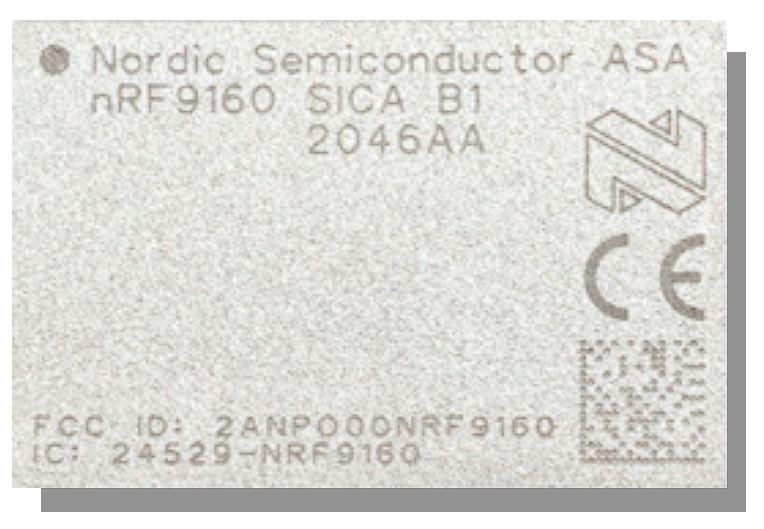
\includegraphics[width=0.3\textwidth]{Include/Figure/Hardware/nRF9160_SiP_chip.png}
	\caption{\textit{nRF9160 SiP} chip - Source: \textsc{Nordic Semi}\cite{nrf9160brief}}
	\label{fig:nRF9160_SiP_chip}
\end{figure}

\subsection{Application domain}

The \textit{nRF9160 SiP}\cite{nrf9160brief} targets asset tracking applications, the \textit{SiP} has a buit-in \textit{nRF Cloud Location Services}\cite{nrfcldlocsrvc} that provide built-in \textit{LTE} and \textit{GNSS} location support with:
\begin{itemize}
\item Assisted \textit{GPS}
\item Predicted \textit{GPS}
\item Single-cell and multi-cell location service
\end{itemize}


The figure \ref{fig:nRF9160_SiP_product_brief} illustrates an application circuit diagram of the \textit{nRF9160 SiP}\cite{nrf9160brief}:

\begin{figure}[H]
	\centering
	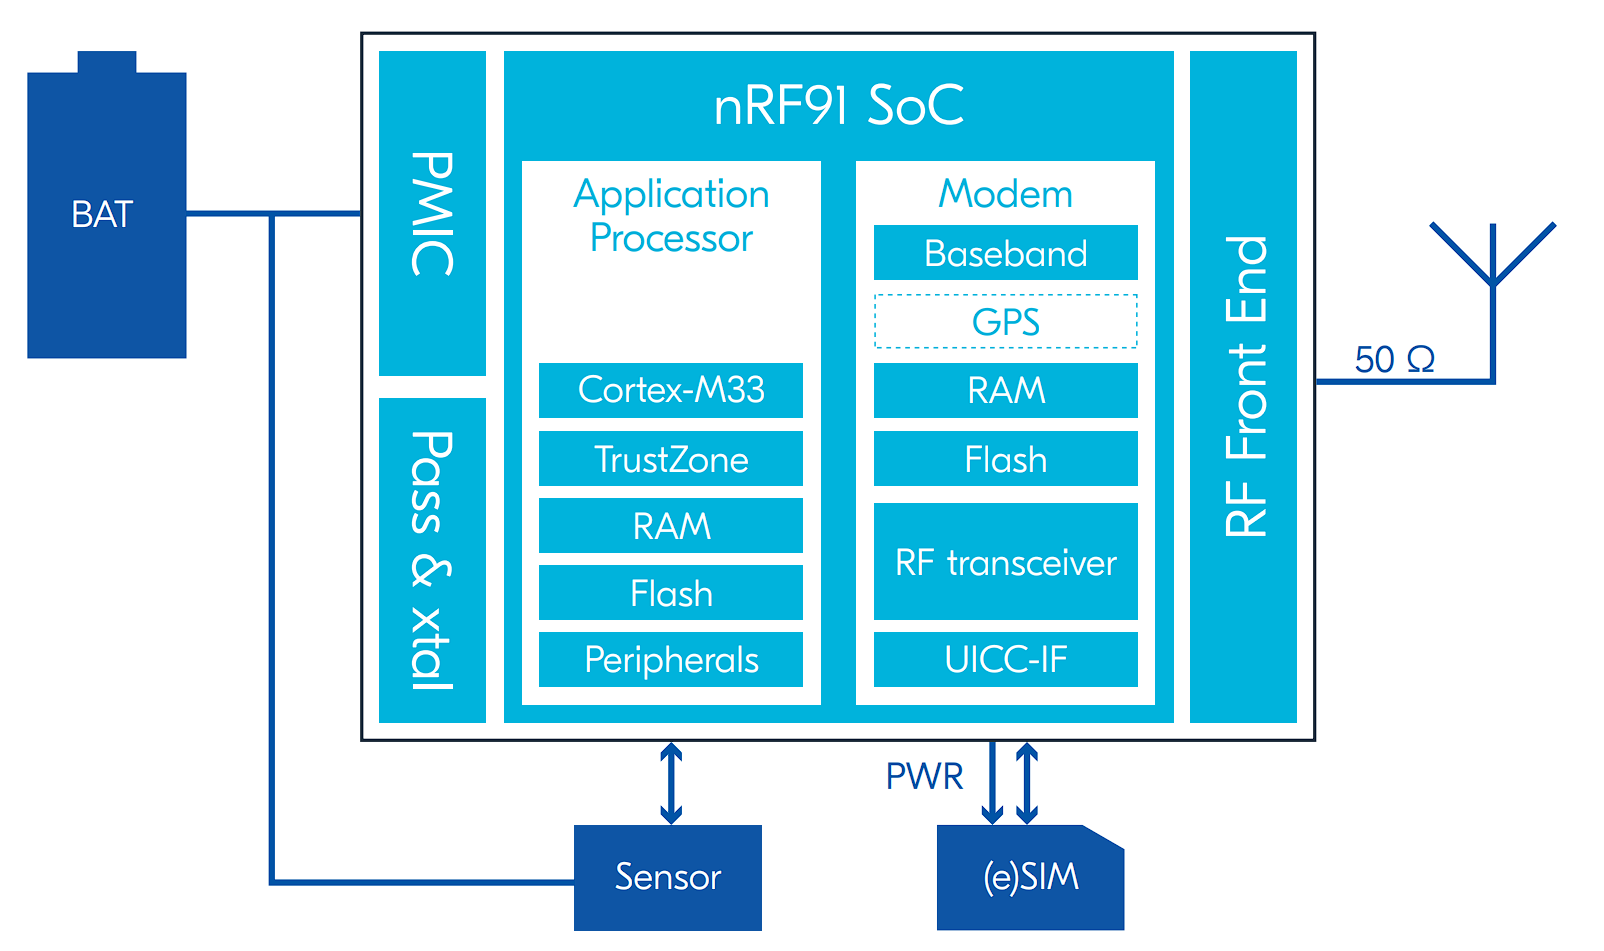
\includegraphics[width=1\textwidth]{Include/Figure/Hardware/nRF9160_SiP_product_brief.png}
	\caption{Application Circuit - Source: \textsc{Nordic Semi}\cite{nrf9160brief}}
	\label{fig:nRF9160_SiP_product_brief}
\end{figure}

With these characteristics, the \textit{nRF9160 SiP} is oriented towards applications such as:
\begin{itemize}
\item Logistics and asset tracking
\item Smart city and smart agriculture
\item Predictive maintenance and industrial
\item Wearables and medical
\end{itemize}

\subsection{\textit{nRF9160 SiP} key features}
The \textit{nRF9160 SiP} offers good performance and many great features for wearable \textit{IoT}, tracking and connected applications.

\subsubsection{\textit{LTE-M}/\textit{NB-IoT} modem}
The \textit{nRF9160 SiP} modem key data are shown in the table \ref{tab:modem}:

\begin{table}[H]
\centering
\begin{tabular}{|l|l|}\hline
Frequency range & $700-2200\si{\mega\hertz}$ \\\hline
Throughput & LTE-M: 3$00$/$375$ kbps \\\hline
(DL/UL) & NB-IoT: $30$/$60$ kbps \\\hline
Output power & Up to $23$ dBm \\\hline
RX sensitivity & \centered{
$\bullet$ LTE-M: $-108$ dBm \\
$\bullet$ NB-IoT: $-114$ dBm \\
$\bullet$ GPS: $-155$ dBm \\
}\\\hline
Mode & HD-FDD \\\hline
\end{tabular}
\caption{\textit{LTE-M}/\textit{NB-IoT} modem key data table\cite{nrf9160brief}}
\label{tab:modem}
\end{table}

\subsubsection{Application processor}
The \textit{nRF9160 SiP} application processor key data are shown in the table \ref{tab:processkd}:

\begin{table}[H]
\centering
\begin{tabular}{|l|l|}\hline
CPU & \SI{64}{\mega\hertz} Arm Cortex-M33 Arm TrustZone \\\hline
Flash & $1$ MB \\\hline
RAM & $256$ KB \\\hline
Security & Arm Cryptocell 310\\\hline
Peripherals & \centered{
$\bullet$ $4\times$SPI/UART/TWI\\
$\bullet$ $4\times$PWM, PDM, I2S\\
$\bullet$ $12$bit/$200$ ksps ADC\\
$\bullet$ $3\times$TIMER, 2xRTC, WDT}\\\hline
\end{tabular}
\caption{Application processor key data table\cite{nrf9160brief}}
\label{tab:processkd}
\end{table}
\;\\[-50pt]
\subsubsection{Current consumption (23 dBm TX power, 3.7 V supply)}
The \textit{nRF9160 SiP} consumption key data are shown in the table \ref{tab:modem}:

\begin{table}[H]
\centering
\begin{tabular}{|l|l|}\hline
PSM floor current & \centered{LTE-M: \SI{2.7}{\micro\ampere}\\ NB-IoT: \SI{2.7}{\micro\ampere}} \\\hline
eDRX, 655 seconds  & \centered{LTE-M: \SI{6}{\micro\ampere}\\ NB-IoT: \SI{9}{\micro\ampere}} \\\hline
\end{tabular}
\caption{Current consumption key data table\cite{nrf9160brief}}
\label{tab:consumption}
\end{table}
\subsubsection{Operating conditions and package}
\textit{nRF9160} operating conditions and package key data are shown in table \ref{tab:modem}:

\begin{table}[H]
\centering
\begin{tabular}{|l|l|}\hline
Supply voltage & $3.0-5.5\si{\volt}$ \\\hline
Temperature & $-40$ to \SI{85}{\celsius}\\\hline
Package & $10\times 16 \times 1.04 \; \si{\milli\meter}$ \textit{LGA} \\\hline
\end{tabular}
\caption{Operating conditions and package key data table\cite{nrf9160brief}}
\label{tab:operatingconditions}
\end{table}

\section{Power Supply}
The battery cell technology choice is a crucial step in the conception of a smart-watch. In order to make the best choice possible, it is necessary to realize the state-of-the-art of available technologies and solutions on market.\\

A crucial step consists in the identification of most relevant constraints of the system, which are:
\begin{itemize}
\item The autonomy of the smart-watch must be sufficient. Approximately one week (5-7 days) of normal usage.
\item The smart-watch must implement a fast charge option. Full charge in 1-2 hours is preferable.
\item The size must be minimal. A maximal diameter of 40 \si{\milli\meter} to 50 \si{\milli\meter} is desirable.
\item Components must be available and price must be as low as possible and as high as necessary.
\end{itemize}

\subsection{Lithium Battery Technologies\cite{litBatTech}}

\subsubsection{Lithium-ion, Lithium Polymer and Lithium Iron Phosphate\cite{litBatTech}}
Currently, lithium is the metal with the highest \textit{energy density} ($\si{\watt\hour\per\kilogram}$) while keeping a very good \textit{power density} ($\si{\watt\per\kilogram}$). This feature still makes lithium the best solution currently available for batteries, especially for small, compact, and lightweight portable applications.

Lithium power source offer interesting advantages if:
\begin{itemize}
\item A higher system voltage is required (i.e. \SI{3.0}{\volt} to \SI{3.9}{\volt} per cell)
\item The system weight must be as low as possible
\item A long shelf life is required
\item The system will be used in a wide range of temperature
\item The system reliability is crucial 
\item The system requires a high energy density
\item The system environmental concerns such as temperature, vibration or shock are high
\item The application requires a continuous source of power for a long period of time\\
\end{itemize}

The main disadvantages of a lithium power source is the price, that is not the cheapest available and the danger of the technologies. Li-Ion and Li-Poly battery doesn't support over charging and over discharging, this can lead to the destruction of the cell with a serious risk of exploding or catching on fire. This is why a battery protection circuit is an obligation while working with that kind of technology. 

\subsubsection{Lithium Batteries\cite{litBatTech}}
Lithium batteries are made with lithium metal or lithium compounds as an anode. They are disposable (primary) batteries that can provide voltages from \SI{1.5}{\volt} to \SI{3.7}{\volt} depending on the design and chemical compounds used. This voltage is over twice the one of an ordinary zinc-carbon battery or alkaline cell battery.

\begin{figure}[H]
	\centering
	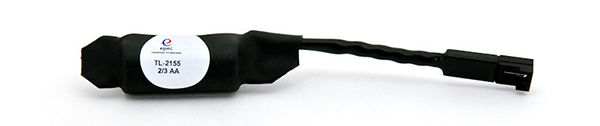
\includegraphics[width=0.6\textwidth]{Include/Figure/Hardware/primary-lithium-battery-pack.jpg}
	\caption{Primary Lithium Battery Pack for Conversion Tracking Device\cite{litBatTech}}
	\label{fig:lithbatpack}
\end{figure}

\subsubsection{Lithium-Ion Batteries\cite{litBatTech}}
Lithium-ion batteries are similar to lithium batteries, except that they are rechargeable. They are common in portable application and consumer electronics because of the following characteristics: 
\begin{itemize}
\item High energy-to-weight ratio
\item No memory effect
\item Slow self-discharge when not in use
\end{itemize}

\begin{figure}[H]
	\centering
	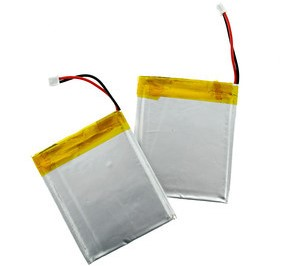
\includegraphics[width=0.4\textwidth]{Include/Figure/Hardware/lithium-ion-battery-pack.jpg}
	\caption{Lithium-Ion Battery Pack for GPS Tracking Device\cite{litBatTech}}
	\label{fig:lithionpack}
\end{figure}

Lithium-ion batteries are made of the three primary functional components:
\begin{itemize}
\item \textbf{Anode:}
	\begin{itemize}
		\item Is the negative electrode
		\item Commercially, is usually made with graphite
	\end{itemize}
\item \textbf{Cathode:} 
	\begin{itemize}
		\item Is the positive electrode
		\item Commercially, is usually made of a layered oxide (such as lithium cobalt oxide), one based on a 					polyanion (such as lithium iron phosphate), or one based on a spinel (such as lithium manganese oxide), 					although materials such as TiS2 (titanium disulfide) originally were also used.
	\end{itemize}
\item \textbf{Electrolyte:} 
	\begin{itemize}
		\item Is a liquid or gel which contains ions and can be decomposed by electrolysis\\
	\end{itemize}
\end{itemize}

Lithium-ion batteries' voltage, capacity, life, and safety can change drastically and is dependent to the choice of material for the anode, cathode and the electrolyte.\\

Lithium-ion battery have the following cycle:
\begin{itemize}
\item \textbf{Discharge:} During the discharge, lithium ions move from the \textit{anode} to the \textit{cathode}
\item \textbf{Charge:} During the charge, lithium ions move from the \textit{cathode} to the \textit{anode}
\end{itemize}

\subsubsection{Lithium Polymer (LiPo)\cite{litBatTech}}

Lithium-ion polymer batteries, polymer lithium-ion, or lithium polymer batteries are also very common rechargeable batteries (secondary cell). They are normally composed of several identical secondary cells in parallel addition to increase the discharge current capability.

\begin{figure}[H]
	\centering
	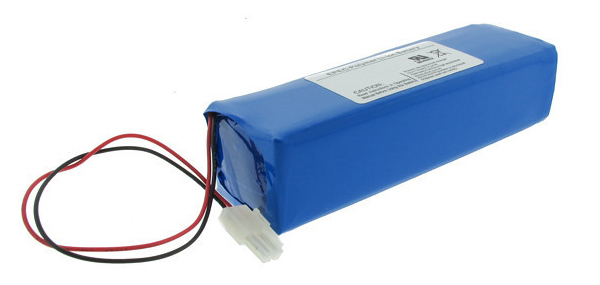
\includegraphics[width=0.7\textwidth]{Include/Figure/Hardware/lithium-polymer-battery-pack.jpg}
	\caption{Lithium Polymer Battery Pack for Medical Application\cite{litBatTech}}
	\label{fig:lithpopack}
\end{figure}

\subsubsection{Lithium Iron Phosphate (LiFePO4)\cite{litBatTech}}
Lithium Iron Phosphate batteries better safety characteristics than Lithium-ion technology, this due to the phosphate based technology, which has better thermal and chemical stability. Phosphate chemistry offers a longer cycle life and are less sensitive during charge and discharge and are incombustible in this situation. They are also more stable under overcharge or short circuit conditions, and they can withstand high temperatures without decomposing. Even when the output current is high, the phosphate based cathode material will not burn and is not prone to thermal runaway.

\subsubsection{Lithium Ion Cathode Chemistry Comparison table}

\begin{table}[H]
\centering
\resizebox{\textwidth}{!}{  
\begin{tabular}{|l|c|c|c|c|}\hline
\centered{Cathode Material}  &
\begin{tabular}{c} Typical \\ Voltage (\si{\volt}) \end{tabular}  &
\begin{tabular}{c} Energy Density \\ Gravimeric \\ (\si{\watt\hour\per\kilogram}) \end{tabular}  &
\begin{tabular}{c} Energy Density \\ Volumetric \\ (\si{\watt\hour\per\liter}) \end{tabular}  &
\begin{tabular}{c} Thermal \\ Stability \end{tabular}  \\ \hline\hline
\centered{Cobalt Oxide} 								& 	3.7	&	195		&	560	&	Poor			\\\hline
\centered{Nickel Cobalt \\ Aluminum \\ Oxide (NCA)} 	&	3.6	&	220		&	600	&	Fair			\\\hline
\centered{Nickel Cobalt \\ Manganese \\ Oxide (NCM)}	&	3.6	&	205		&	580	&	Fair			\\\hline
\centered{Manganese \\ Oxide (Spinel)}				&	3.9	&	150		&	420	&	Good			\\\hline
\centered{Iron Phosphate \\ (LFP)}					& 	3.2	&	90-130	&	333	&	Very Good	\\\hline
\end{tabular}}
\caption{Lithium Ion Cathode Chemistry Comparison table\cite{litBatTech}}
\label{tab:litBatTech}
\end{table}

\subsubsection{Conclusion}
Currently, optimal power density and a compact power supply are synonym of lithium battery technology. The Principal advantages and applications constraints of lithium power sources are :
\begin{itemize}
\item Offer high output voltage : \SI{3.0}{\volt} to \SI{3.9}{\volt} per cell
\item Have one of the best Gravimetric energy density \si{[\watt\hour\per\kilo\gram]} available on market
\end{itemize}
However, lithium-ion battery always requires a protection circuit to manage its charge and discharge in order to maximize its usage safety. Therefore, a special attention must be given to the battery management circuit and the right choice of battery capacity, charge and discharge current and the system load when implementing a lithium-ion battery.

\subsection{Battery - State of art}

In order to keep a reasonable size for the smart-watch, its diameter must be smaller than \SI{50}{\milli\meter} with an ideal diameter sitting around \SI{45}{\milli\meter}. It has also been decided with Medard Rieder and Patrice Rudaz to choose a circular shape for the design of the smart-watch.\\

In order to implement the maximum autonomy possible in the system, the best idea seems to select a circular (round) battery cell with a diameter fitting inside the smart-watch's diameter of \SI{45}{\milli\meter}.\\

After some researches on the market, two solutions seemed to correspond to those needs:
\begin{enumerate}
\item Lithium-ion Rechargeable Coin Cell Battery
\item Round LiPo Battery Cells
\end{enumerate}

\subsubsection{Lithium Ion Rechargeable Coin Cell Battery}

Lithium-ion Rechargeable Coin Cell Battery are small lithium-ion battery package in common button cell and coin cell batteries standards. The package is labeled similarly to the non-rechargeable primary coin/button cell battery. The code consists of two letters, followed by three or four numbers. This standard correspond to the \textsc{International Electrotechnical Commission} (\textit{IEC}). However, there are still coin/button cells that correspond to an older standard which has different naming.\\

The standard only describes primary batteries. Rechargeable types have a different prefix that is not in the IEC standard, for example ML, RJD and LiR button cells use rechargeable lithium technology.

\begin{table}[H]
\centering
\begin{tabular}{|c|c|c|c|}\hline
\centered{Battery \\ Type} & \centered{Shape} & \centered{Diameter\\ \si{[\milli\meter}]} & \centered{Height \\$[\si{\milli\meter}/10]$} \\ \hline
LI & R & 24 & 50 \\ \hline
\end{tabular}
\caption{Coin/Button cell battery \textsc{IEC} standard}
\end{table}

The figure \ref{fig:LIR2450} illustrates lithium-ion rechargeable coin cells with the following label:
\begin{itemize}
\item \textit{LI}: Rechargeable lithium-ion technology
\item \textit{R}: Round (circular) shaped battery
\item $24$: The battery cell diameter is $24.5\si{\milli\meter} \pm 0.50 \si{\milli\meter}$
\item $50$: The battery cell height is \SI{5}{\milli\meter} tall
\end{itemize}

\begin{figure}[H]
\centering
\begin{subfigure}{.4\textwidth}
	\centering
	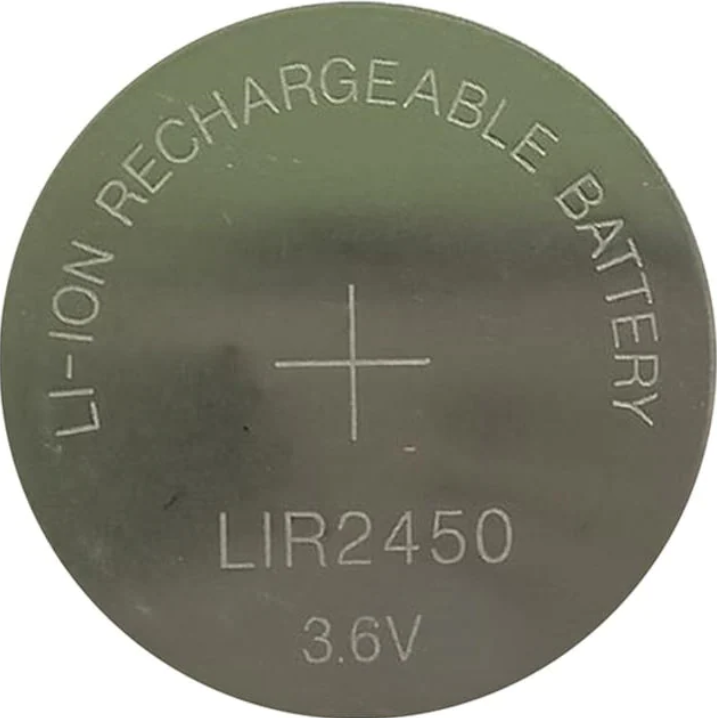
\includegraphics[width=0.35\textwidth]{Include/Figure/Hardware/LIR2450.png}
\end{subfigure}
\begin{subfigure}{.4\textwidth}
	\centering
	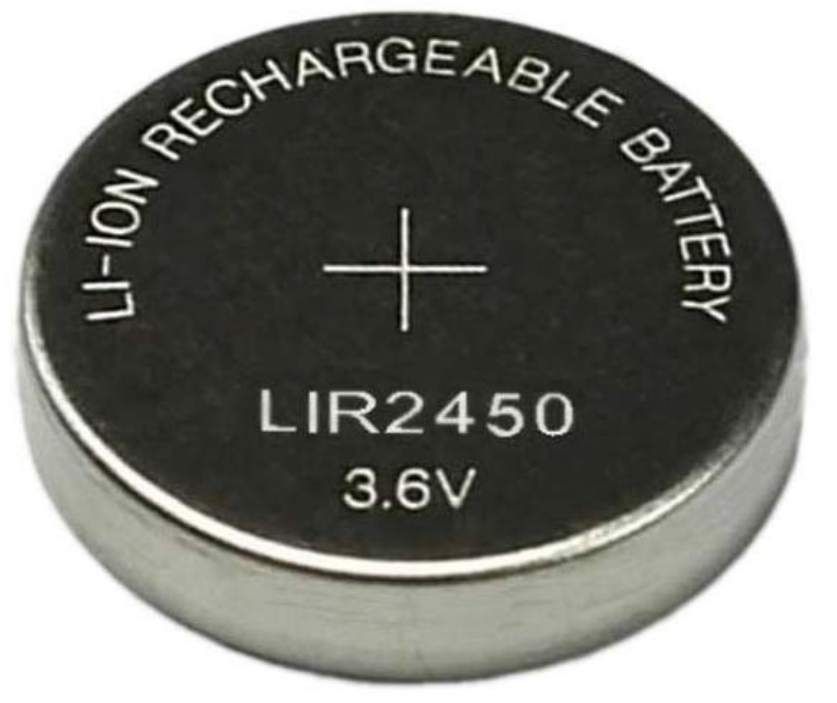
\includegraphics[width=0.4\textwidth]{Include/Figure/Hardware/LIR2450_2.png}
\end{subfigure}
	\caption{Lithium Ion Rechargeable Coin Cell Battery\cite{LIR2450}}
	\label{fig:LIR2450}
\end{figure}


\textsc{CDE} / \textsc{Illinois Capacitor RJD} provide multiple model of "high capacity" lithium-ion rechargeable coin cell battery. They claim that their batteries offer "a reduced risk of overheating compared to conventional coin-cell batteries."\cite{LIR2450}.\\

RJD batteries claims the following characteristics:
\begin{itemize}
\item A nominal voltage of \SI{3.7}{\volt} (\SI{4.2}{\volt} to \SI{3.0}{\volt})
\item A charging time $<$ \SI{3}{\hour}
\item High-power rating batteries: graphite anodes and lithium nickel manganese cobalt oxide cathode
\item Ideal for memory backup circuits, electronic wearables, and Internet of Things (IoT) devices\\
\end{itemize} 

The figure \ref{fig:rjd_standard_coin_cell_options} illustrate the standard coin cell options from \textsc{RJD}:

\begin{figure}[H]
	\centering
	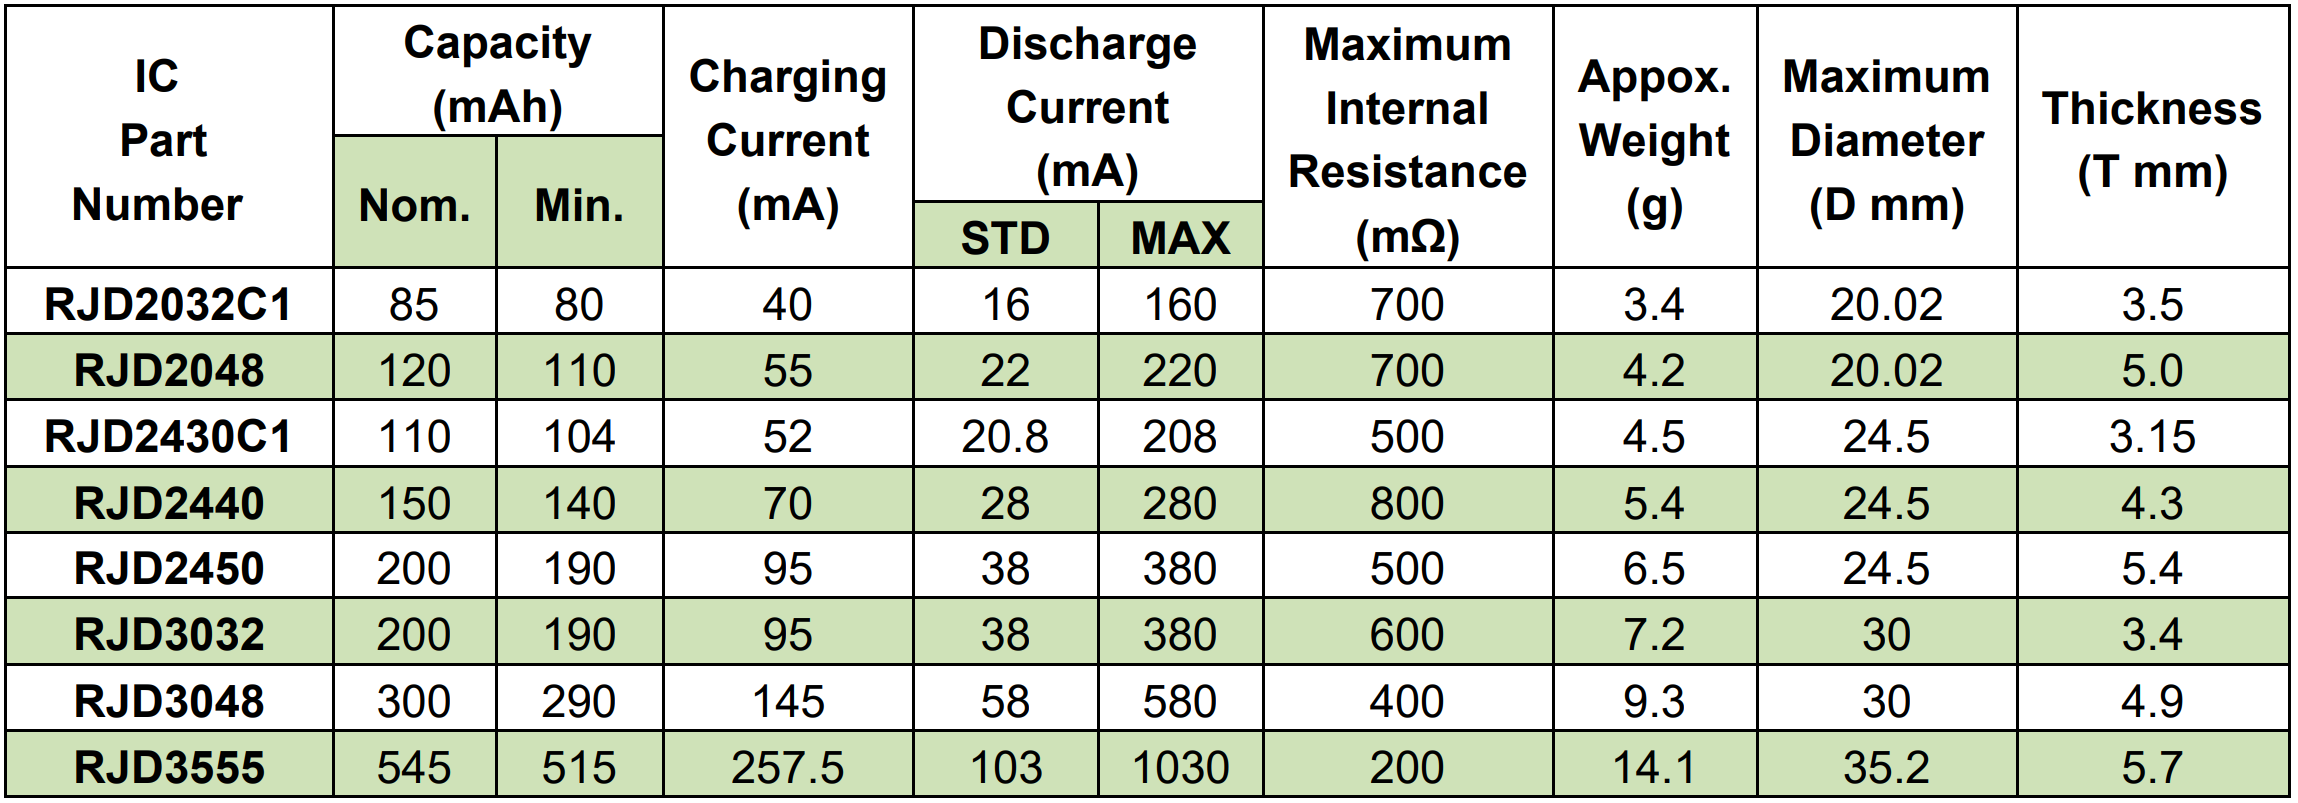
\includegraphics[width=1\textwidth]{Include/Figure/Hardware/rjd_standard_coin_cell_options.png}
	\caption{RJD - Standard Coin Cell Options\cite{rjdLiIon}}
	\label{fig:rjd_standard_coin_cell_options}
\end{figure}

The figure \ref{fig:rjd_cell_dimensions} illustrate corresponding dimensions:


\begin{figure}[H]
	\centering
	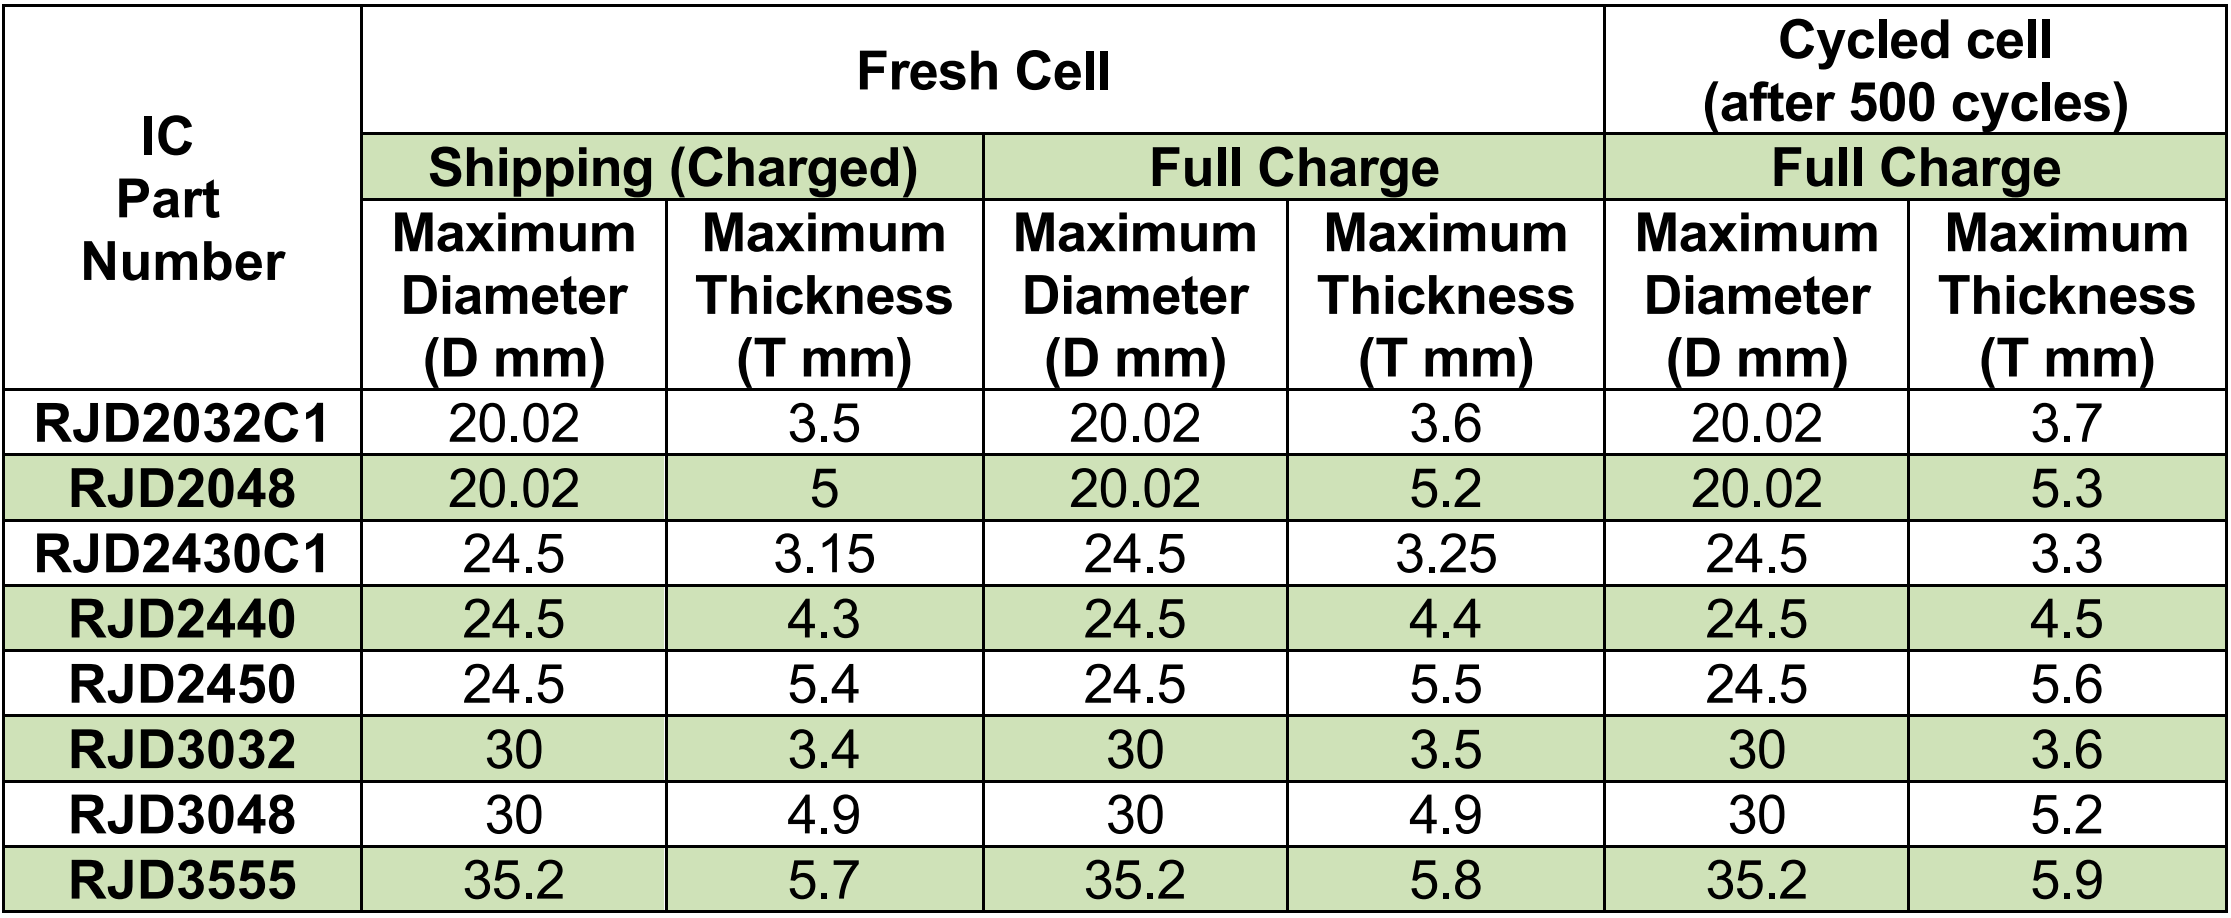
\includegraphics[width=1\textwidth]{Include/Figure/Hardware/rjd_cell_dimensions.png}
	\caption{RJD - Standard Coin Cell Dimensions\cite{rjdLiIon}}
	\label{fig:rjd_cell_dimensions}
\end{figure}

\begin{flushleft}
\textbf{Positive points about RJD Battery:}
\end{flushleft}
\begin{itemize}[\textcolor{mygreen}{+}]
\item Compatible with coin cell battery socket and standards
\item Available in a wide range of diameter: from \SI{20}{\milli\meter} to \SI{35}{\milli\meter} 
\item Available in a wide range of thickness: from \SI{3.5}{\milli\meter} to \SI{5.7}{\milli\meter} 
\item Offer multiple choice of capacity: from \SI{85}{\milli\ampere\hour} to \SI{545}{\milli\ampere\hour}
\item Relatively cheap: \SI{100}{[\milli\ampere\hour]} $\approx 6.24$ \$
\item Easily available (\url{mouser.ch},\url{digikey.com}, etc...)
\item Sufficient discharge current: from \SI{580}{\milli\ampere} to  \SI{1030}{\milli\ampere} (for the two interesting models)
\end{itemize}

\pagebreak

\begin{flushleft}
\textbf{Negative points about RJD Battery:}
\end{flushleft}
\begin{itemize}[\textcolor{red}{-}]
\item Only two interesting models: \textit{RJD3048} (\SI{300}{[\milli\ampere\hour]}) and \textit{RJD3555} (\SI{545}{[\milli\ampere\hour]})
\item Relatively small capacity: maximum capacity of \SI{545}{[\milli\ampere\hour]}
\item Require a mounting socket which increase the battery clutter in the system
\item Relatively slow recharging time $\sim \SI{3}{\hour}$
\end{itemize}

\subsubsection{Round LiPo Battery Cells}

While LiPo battery have a slightly lower energy density than lithium-ion, it offers many interesting characteristics such as slimmer package and a wider range of shapes sand sizes. LiPo are also widely available and relatively cheap. LiPo battery offers an interesting alternative to lithium-ion rechargeable coin battery.

\begin{figure}[H]
	\centering
	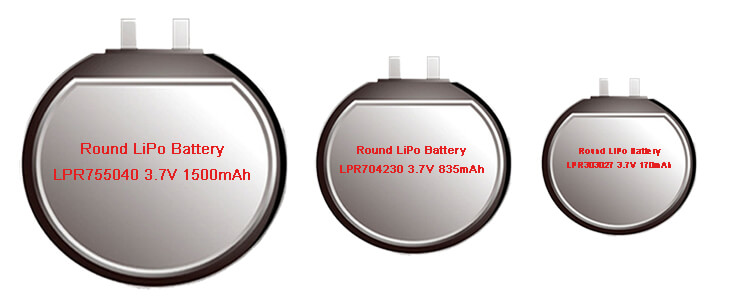
\includegraphics[width=0.6\textwidth]{Include/Figure/Hardware/Round-LiPo-Batteries.jpg}
	\caption{Round LiPo Battery Cells\cite{roundLipoCell}}
	\label{fig:RoundLiPoBatteries}
\end{figure}

\begin{flushleft}
\textbf{LiPo battery cells main features:}
\end{flushleft}
\begin{itemize}
\item Round shape allow a higher energy density with an optimized compact design
\item Nominal voltage from \SI{3.6}{\volt} to \SI{3.8}{\volt}
\item If required, PCM, NTC and connector can be easily assembled to the battery
\item A wide range of available capacity from \SI{135}{\milli\ampere\hour} to \SI{1500}{\milli\ampere\hour}
\item Low self discharge and a longer cell's life
\end{itemize}

\textbf{\textsc{LiPol Battery Co. Ltd ®} Round LiPo Battery Cell options:}

\begin{table}[H]
\centering
\begin{tabular}{|l|c|c|c|}\hline
Part No.		&	Voltage 	&	Capacity		&	Size		\\\hline
LPR403535	&	3.7V 	&	390mAh		&	4.0x35mm \\\hline
LPR433736	&	3.8V 	&	530mAh		&	4.3x37mm \\\hline
LPR443535	&	3.7V 	& 	450mAh		&	4.4x35mm \\
LPR443735	&	3.7V 	& 	450mAh		&	4.4x37mm \\\hline
LPR453535	&	3.7V 	& 	450mAh		&	4.5x35mm \\
LPR453535	&	3.8V 	& 	475mAh		&	4.5x35mm \\
LPR453535	&	3.8V 	& 	490mAh		&	4.5x35mm \\\hline
LPR463535	&	3.8V 	& 	480mAh		&	4.6x35mm \\\hline
LPR473736	&	3.8V 	& 	580mAh		&	4.7x37mm \\\hline
LPR483535	&	3.8V 	& 	530mAh		&	4.8x35mm \\\hline
\end{tabular}
\caption{Round LiPo Battery Cells Table - Part 1 - Source:\cite{roundLipoCell}}
\label{tab:roundLipoCell1}
\end{table}

\begin{table}[H]
\centering
\begin{tabular}{|l|c|c|c|}\hline
Part No.		&	Voltage 	&	Capacity		&	Size		\\\hline
LPR503027	&	3.7V 	& 	300mAh		&	5.0x30mm \\\hline
LPR533535	&	3.8V 	& 	560mAh		&	5.3x35mm \\\hline
LPR543535	&	3.8V 	&	610mAh		&	5.4x35mm \\\hline
LPR553532	&	3.8V 	& 	600mAh		&	5.5x35mm \\
LPR553535	&	3.7V 	& 	580mAh		&	5.5x35mm \\
LPR553535	&	3.7V 	& 	600mAh		&	5.5x35mm \\\hline
LPR603533	&	3.7V 	& 	630mAh		&	6.0x35mm \\
LPR603535	&	3.8V 	& 	650mAh		&	6.0x35mm \\
LPR604543	&	3.7V 	& 	1050mAh		&	6.0x45mm \\\hline
LPR653027	&	3.8V 	& 	430mAh		&	6.5x30mm \\
LPR653929	&	3.8V 	& 	665mAh		&	6.5x39mm \\\hline
\end{tabular}
\caption{Round LiPo Battery Cells Table - Part 2 - Source:\cite{roundLipoCell}}
\label{tab:roundLipoCell2}
\end{table}

\subsubsection{Selected Battery - 503535 3.8v 580mAh round lipo battery cells}

The context of Master thesis requires to find quick and available solution and does not allow ordering custom product. Furthermore, batteries are considerate of hazardous materials and are not very easy to deliver.\\

Because of this context, the choice available was considerably reduced. A suitable solution is the component "\textit{503535 3.8v 580mAh round lipo battery cells}" available on \url{https://batteryzone.de/products/503535-580mah-hochspannung-3-8v-runde-polymer-smart-watch-moxibustion-instrument-auto-smart-box-batterie?_pos=1&_sid=59cfd2d74&_ss=r}\\

The selected battery is illustrated on the figure \ref{fig:503535RLipo}.

\begin{figure}[H]
	\centering
	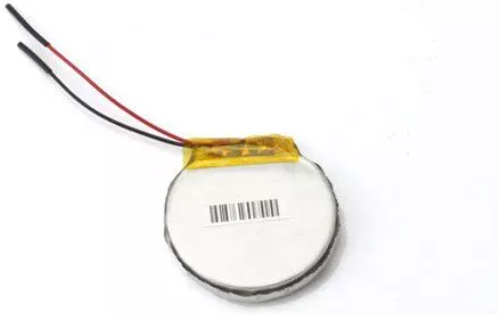
\includegraphics[width=0.6\textwidth]{Include/Figure/Hardware/503535RLipo.png}
	\caption{503535 3.8v 580mAh round lipo battery cells \cite{503535RLipo}}
	\label{fig:503535RLipo}
\end{figure}

\pagebreak

\textbf{Basic Information :}

The selected battery is not the most ideal choice, because it is not the thinner model available, but it has a big capacity and a fitting diameter of \SI{35}{\milli\meter}.\\

The selected battery has the following characteristics:
\begin{table}[H]
\centering
\begin{tabular}{|l|l|c|}\hline
Cell Thickness 		&	$5.0 \pm 0.2$	& $\si{[\milli\meter]}$\\
Cell Diameter 		&	$35 \pm 0.5$ 	& 	$\si{[\milli\meter]}$\\
Charge voltage		&	$4.35 \pm 0.03$	&	$\si{[\volt]}$\\
Nominal voltage		&	$3.8$ 			&	$\si{[\volt]}$\\
Nominal capacity		&	$580$			&	$\si{[\milli\ampere\hour]}$\\
Fully charge voltage	&	$4.35$ 			&	$\si{[\volt]}$\\
Ship out voltage		&	$3.9 - 4.2 $		&	$\si{[\volt]}$\\\hline
\end{tabular}
\caption{503535 $3.8\si{\volt}$ $580\text{mAh}$ round lipo - Basic Information \cite{roundLipoCell}}
\label{tab:503535RLipo_basic_info}
\end{table}

\textbf{Battery detailed specification :}
\begin{table}[H]
\centering
\begin{tabular}{|l|l|c|}\hline
Charge current 				&	\centered{Standard Charging: $0.2$C ($116$) \\ Rapid charge: $1.0$C ($580$)} & \si{[\milli\ampere]}\\ \hline
Charging method				& \centered{Charge with constant current\\ $0.2$C to \SI{4.2}{\volt}, then charge \\ with constant voltage \SI{4.2}{\volt} \\ till until charge current\\ is less than $0.01$C} & [ - ]\\ \hline
Standard discharge current	&	\centered{$0.2$C ($116$)} 	& 	\si{[\milli\ampere]}\\ \hline
Max.discharge current		&	\centered{$1$C  ($580$)}		& 	\si{[\milli\ampere]}\\ \hline
Discharge cut-off voltage	& 	\centered{$3.0$} 			& 	\si{[\volt]}\\\hline
Operating environment		&	\centered{Charging: $0\sim 45$ \\ Discharging: $-20\sim 60$} & \si{[\celsius]}\\\hline
Storage temperature			& 	\centered{less than one month: $-20\sim 40$ \\less than half year: $-20\sim 30$} & \si{[\celsius]}\\\hline
PCB \& Wires \& connector	&	\centered{Optional}			& 	[ - ]\\ \hline
Cycles						&	\centered{$500$}				&	[times]\\ \hline
Warranty						&	\centered{$12$} 				&	[months]\\\hline
\end{tabular}
\caption{503535 \SI{3.8}{\volt} \SI{580}{[\milli\ampere\hour]} round lipo - Battery specification \cite{roundLipoCell}}
\label{tab:503535RLipo_basic_info}
\end{table}

\pagebreak

\section{Introduction to \textit{GNSS}}

The website \url{www.gps.gov}\cite{gnssDef} describes \textit{GNSS} as a general term describing any satellite constellation providing \textit{PNT} services on a global or regional basis:
\begin{enumerate}
\item Positioning \textit{(P)}
\item Navigation \textit{(N)}
\item Timing \textit{(T)}\\
\end{enumerate}

The most prevalent \textit{GNSS} is \textbf{GPS} (\textit{Global Positioning System}) which is the utility owned by the United States with 24 satellites, but it exists several others \textit{PNT} utilities available to provide complementary and independent \textit{PNT} capability.

\begin{flushleft}
The mains other \textit{PNT} utilities are:
\end{flushleft}

\begin{enumerate}
\item \textbf{BeiDou} \textit{Navigation Satellite System (BDS)}: Global \textit{GNSS} owned and operated by the People's Republic of China (\textit{PRC}) with 30 satellites.
\item \textbf{Galileo}: Global \textit{GNSS} owned and operated by the European Union (\textit{UE}) with 30 satellites.
\item \textbf{GLONASS} \textit{Globalnaya Navigazionnaya Sputnikovaya Sistema} (Global Navigation Satellite System): Global \textit{GNSS} owned and operated by the Russian Federation with 24 satellites.
\item \textbf{IRNSS/NavIC} \textit{Indian Regional Navigation Satellite System / Navigation Indian Constellation} Global \textit{GNSS} owned and operated by the Government of India with 7 satellites. \textit{IRNSS} is an autonomous system designed to cover the Indian region and \SI{1500}{\kilo\meter} around the Indian mainland.
\item \textbf{QZSS} \textit{Quasi-Zenith Satellite System}: Global \textit{GNSS} owned by the Government of Japan and operated by \textit{QZS} System Service Inc. (\textit{QSS}) with 5 satellites.
\end{enumerate}

\section{Introduction to Cellular IoT}

\subsection{Introduction to \textit{LTE}}
\;\\[-35pt]
\begin{figure}[H]
\centering

\includegraphics[width=0.15\textwidth]{Include/Figure/research/3GPP_LTE_logo.png}
\caption{\textit{LTE} Logo\cite{LTE}}
\label{fig:ltelogo}
\end{figure}

Long-Term Evolution (\textit{LTE}\cite{LTE}) is a wireless broadband communication and data terminals standard for mobile devices. \textit{LTE} is based on the \textit{GSM}/{EDGE} and the \textit{UMTS}/{HSPA} standards. Frequencies and bands of \textit{LTE} differ from country to country, which implies that to use \textit{LTE} in all countries where it is supported, it is mandatory to use multi-band receivers. 

\subsection{Description of \textit{LTE-M}}

\textsc{Nordic Semi.} provides a good introduction to \textit{LTE-M} on their website\cite{LTEM_NBIOT}:

\begin{figure}[H]
\centering
\textbf{
\includegraphics[width=0.4\textwidth]{Include/Figure/research/LTEM_logo.png}
\caption{\textit{LTE-M} Logo\cite{LTE}}}
\label{fig:ltemlogo}
\end{figure}

Low-power application required a mode fitting alternative to regular \textit{LTE}, \textit{LTE-M} that is also known as \textit{Cat-M1} is specifically design for medium throughput requirement and low-power application. \textit{LTE-M} has a bandwidth of \SI{1.4}{\mega\hertz}, which significantly narrower than regular \textit{LTE} with \SI{20}{\mega\hertz}. This gives a longer range to \textit{LTE-M} by sacrificing throughput providing approximately \SI{100}{k b p s} application throughput running IP with the following performances:
\begin{itemize}
\item \textbf{Uplink} : \SI{375}{k b p s}
\item \textbf{Downlink} : \SI{300}{k b p s} 
\end{itemize}

\begin{flushleft}
\textbf{Main advantages of \textit{LTE-M}:}
\end{flushleft}
\begin{enumerate}
\item Suitable for \textit{TCP}/{TLS} end-to-end secure connections.
\item Fully supports mobility by using the same cell handover features as regular \textit{LTE}.
\item Roaming is currently available, meaning it is suitable for multiple regions operating applications.
\item Suitable for time-critical applications offering real-time communication with latency in the millisecond range.
\item Suitable for applications requiring: medium-throughput, low power, low latency and mobility.
\item Perfect for applications, such as: asset tracking, wearable, medical, \textit{POS} and home security.
\end{enumerate}


\subsection{Description of \textit{NB-IoT}}

\textsc{Nordic Semi.} provides a good introduction to \textit{NB-IoT} on their website\cite{LTEM_NBIOT}:

\begin{figure}[H]
\centering
	\includegraphics[width=0.4\textwidth]{Include/Figure/research/NBIOT_logo.png}
	\caption{\textit{NB-IoT} Logo\cite{LTEM_NBIOT}}
\label{fig:nbiotlogo}
\end{figure}

Applications with even lower throughput requirement needs a solution more fitting than \textit{LTE-M} in order to reduce power consumption. \textit{NB-IoT} that is also known as \textit{Cat-NB1} was specially design for that kind of applications. It has a drastically narrower bandwidth of \SI{200}{\kilo\hertz} providing longer range and lower throughput compared to \textit{LTE-M} and regular \textit{LTE} with the following performances:
\begin{itemize}
\item \textbf{Uplink} : \SI{60}{k b p s}
\item \textbf{Downlink} : \SI{30}{k b p s} 
\end{itemize}
\textit{NB-IoT} technology standard that does not use a traditional \textit{LTE} physical layer but is designed to operate in or around \textit{LTE} bands and coexist with other \textit{LTE} devices.

\begin{flushleft}
\textbf{Main advantages of \textit{NB-IoT}:}
\end{flushleft}
\begin{enumerate}
\item Suitable for: static, low throughput applications requiring low power and long-range.
\item Perfect for applications, such as: smart metering, smart agriculture and smart city applications. 
\item It also provides better penetration in confined environments, like cellars and parking garages, compared to \textit{LTE-M}.
\item If the network supports it and with \textit{Cat-NB2} in \textit{3GPP} release 14 a better throughput can be achieved:
\begin{itemize}
\item \textbf{Uplink} : \SI{169}{k b p s}
\item \textbf{Downlink} : \SI{127}{k b p s} 
\end{itemize}
\end{enumerate}

\section{MQ Telemetry Transport (\textit{MQTT}) Protocol}

\subsection{Description of \textit{MQTT}}
\;\\[-35pt]
\begin{figure}[H]
\centering
	
\includegraphics[width=0.4\textwidth]{Include/Figure/research/mqtt_logo.png}
	\caption{\textit{MQTT} Logo\cite{MQTT}}
\label{fig:nbiotlogo}
\end{figure}

MQ Telemetry Transport (\textit{MQTT}\cite{MQTT}) is a lightweight machine to machine network protocol, using \textit{publish–subscribe} messaging pattern and intended for \textit{message queue} and \textit{message queuing} service. The \textit{MQTT} protocol is designed for connections to remote locations hosting constrained resources or limited network bandwidth devices. This protocol must run over a transport protocol that provides ordered, lossless and bidirectional connections, like \textit{TCP/IP}. \textit{MQTT} is very common and is an open \textit{OASIS} standard and an \textit{ISO} recommendation (\textit{ISO/IEC 20922}).

\subsection{Overview}

\begin{flushleft}
The \textit{MQTT} protocol defines two types of network entities (src.\cite{MQTT}):
\end{flushleft}
\begin{enumerate}
\item \textbf{Broker:} Server receiving all messages from the clients and then routes the messages to the registered clients
\item \textbf{Client:} Device running \textit{MQTT} and connected to a broker over a network
\end{enumerate}

\begin{flushleft}
The main advantages of \textit{MQTT} broker usage are (src.\cite{MQTT}):
\end{flushleft}
\begin{enumerate}
\item Can eliminate vulnerable and insecure client connections. 
\item Can easily be scaled from a single device to many.
\item Can manage and tracks all client connection states, including security credentials and certificates.
\item Can reduce network strain without compromising the security.
\end{enumerate}

\subsection{Protocol Working Principle}
\begin{flushleft}
Working principle of \textit{MQTT} protocol is the following (src.\cite{MQTT}):
\end{flushleft}

\begin{enumerate}
\item \textbf{Data are stored and organized in a defined hierarchy of topics}.
\item \textbf{If a publisher wants to distribute a new item of data:}
\begin{itemize}
\item Publisher sends a control message containing the data to a broker's topic.
\item Broker then distributes the information to any clients that have subscribed to the concerned topic.
\item Publisher does not need to know anything about the number or locations of subscribers.
\item Subscribers do not need to know anything about publishers.
\end{itemize}
\item \textbf{If a broker receives a message on a topic with no subscribers:}
\begin{itemize}
\item It will discard the message unless the publisher of the message designated the message as a retained message.
\end{itemize}
\item \textbf{Retained message:}
\begin{itemize}
\item Is a normal \textit{MQTT} message with the retained flag set to \codeword{true}.
\item Broker stores last retained message and \textit{QoS} for the selected topic.
\item Each client that subscribes to a topic pattern that matches the topic of the retained message receives it immediately after they subscribe.
\item This allows new subscribers to a topic to receive the latest value rather than waiting for a next update from a publisher.
\item The broker can only store a single retained message per topic.
\end{itemize}
\item \textbf{When a publishing client connects for the first time to a broker:}
\begin{itemize}
\item It can set up a default message to be sent to subscribers if the broker detects an unexpected disconnection of the publishing client from it.
\end{itemize}
\item \textbf{Clients only interact with a broker:}
\begin{itemize}
\item A system can contain several broker servers that exchange data based on their current subscribers' topics.
\end{itemize}
\item \textbf{Control message:}
\begin{itemize}
\item A control message can be as little as two bytes of data.
\item If needed, a control message can carry nearly $256$ megabytes of data.
\end{itemize}
\item \textbf{\textit{MQTT} uses fourteen defined message types:}
\begin{itemize}
\item To connect and disconnect a client from a broker
\item To publish data
\item To acknowledge the reception of data
\item To supervise the connection between client and server
\end{itemize}
\item \textbf{Data transmission protocol:}
\begin{itemize}
\item Relies on the \textit{TCP} protocol for data transmission. 
\item A variant, \textit{MQTT-SN}, is used over other transports such as \textit{UDP} or \textit{Bluetooth}.
\end{itemize}
\item \textbf{Security:}
\begin{itemize}
\item Does not include any measures for security or authentication, and connection credentials are in plain text format.
\item Can use \textit{TLS} to encrypt and protect the transferred information against interception, modification or forgery.
\item The default unencrypted port is $1883$.
\item The default encrypted port is $8883$.
\end{itemize}
\end{enumerate}

\pagebreak
\subsection{Message Types}

Figure \ref{fig:mqtt_message_type} illustrates an example of \textit{MQTT} connection (\textit{QoS $0$}) with connect, publish/subscribe and disconnect from client \textit{A}, and also storing of retain messages from the client \textit{B}:

\begin{figure}[H]
\centering
	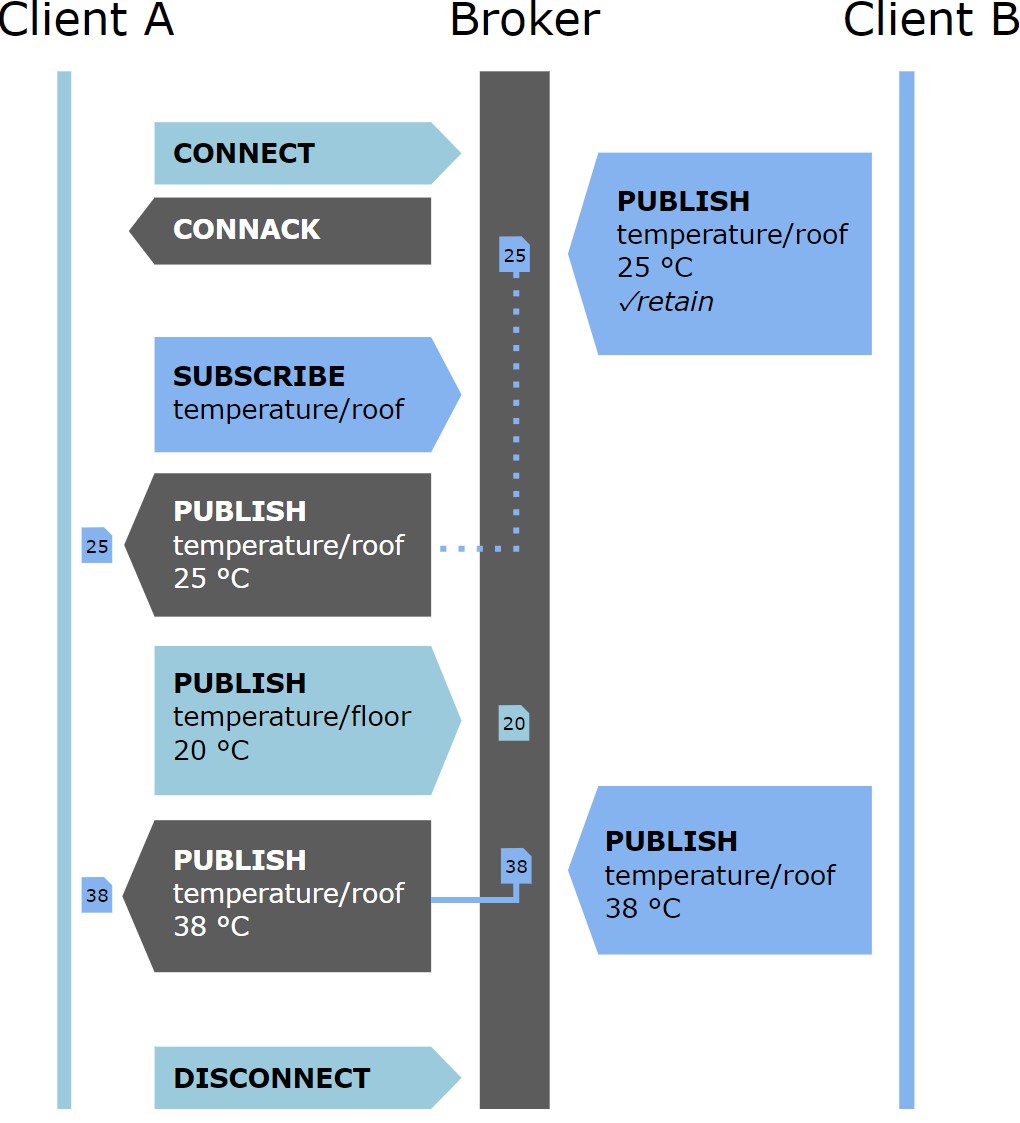
\includegraphics[width=0.6\textwidth]{Include/Figure/research/mqtt_message_type.png}
	\caption{Example of an MQTT connection - Source: \cite{MQTT}}
\label{fig:mqtt_message_type}
\end{figure}

Figure \ref{fig:mqtt_message_type} illustrates the three message types described below:
\begin{itemize}
\item \textbf{Connect:} Waits establishment of a connection with the server and creates a link between the nodes.
\item \textbf{Disconnect:} Waits for the end of any current work of the \textit{MQTT} client, and for disconnection of the \textit{TCP/IP} session.
\item \textbf{Publish:} Immediately returns to the application thread after the request is passed to the \textit{MQTT} client.

\end{itemize}

\end{document}
